\PassOptionsToPackage{unicode=true}{hyperref} % options for packages loaded elsewhere
\PassOptionsToPackage{hyphens}{url}
%
\documentclass[]{article}
\usepackage{lmodern}
\usepackage{amssymb,amsmath}
\usepackage{ifxetex,ifluatex}
\usepackage{fixltx2e} % provides \textsubscript
\ifnum 0\ifxetex 1\fi\ifluatex 1\fi=0 % if pdftex
  \usepackage[T1]{fontenc}
  \usepackage[utf8]{inputenc}
  \usepackage{textcomp} % provides euro and other symbols
\else % if luatex or xelatex
  \usepackage{unicode-math}
  \defaultfontfeatures{Ligatures=TeX,Scale=MatchLowercase}
\fi
% use upquote if available, for straight quotes in verbatim environments
\IfFileExists{upquote.sty}{\usepackage{upquote}}{}
% use microtype if available
\IfFileExists{microtype.sty}{%
\usepackage[]{microtype}
\UseMicrotypeSet[protrusion]{basicmath} % disable protrusion for tt fonts
}{}
\IfFileExists{parskip.sty}{%
\usepackage{parskip}
}{% else
\setlength{\parindent}{0pt}
\setlength{\parskip}{6pt plus 2pt minus 1pt}
}
\usepackage{hyperref}
\hypersetup{
            pdfauthor={Zhenghong Lieu},
            pdfborder={0 0 0},
            breaklinks=true}
\urlstyle{same}  % don't use monospace font for urls
\usepackage{graphicx,grffile}
\makeatletter
\def\maxwidth{\ifdim\Gin@nat@width>\linewidth\linewidth\else\Gin@nat@width\fi}
\def\maxheight{\ifdim\Gin@nat@height>\textheight\textheight\else\Gin@nat@height\fi}
\makeatother
% Scale images if necessary, so that they will not overflow the page
% margins by default, and it is still possible to overwrite the defaults
% using explicit options in \includegraphics[width, height, ...]{}
\setkeys{Gin}{width=\maxwidth,height=\maxheight,keepaspectratio}
\setlength{\emergencystretch}{3em}  % prevent overfull lines
\providecommand{\tightlist}{%
  \setlength{\itemsep}{0pt}\setlength{\parskip}{0pt}}
\setcounter{secnumdepth}{0}
% Redefines (sub)paragraphs to behave more like sections
\ifx\paragraph\undefined\else
\let\oldparagraph\paragraph
\renewcommand{\paragraph}[1]{\oldparagraph{#1}\mbox{}}
\fi
\ifx\subparagraph\undefined\else
\let\oldsubparagraph\subparagraph
\renewcommand{\subparagraph}[1]{\oldsubparagraph{#1}\mbox{}}
\fi

% set default figure placement to htbp
\makeatletter
\def\fps@figure{htbp}
\makeatother

\usepackage{booktabs}
\usepackage[]{natbib}
\bibliographystyle{plainnat}

\author{Zhenghong Lieu}
\date{}

\begin{document}

\hypertarget{introduction}{%
\subsection{Introduction}\label{introduction}}

Good job today. To reiterate, basically I think your research question
should be something like: ``Research shows that districts that consist
of more homogeneous groups of voters achieve better representation on
several dimensions. Meanwhile, many statutes require that districts
be''compact``, a term with many interpretations. It is not clear,
however, that more compact districting plans (however compactness is
measured) result in more homogeneous districts. Are compactness and
homogeneity fundamentally conflicting goals? Are some measures of
compactness more consistent with homogeneity than others?''

\hypertarget{my-contribution}{%
\subsubsection{My contribution}\label{my-contribution}}

\begin{itemize}
\tightlist
\item
  i develop the human compactness metric
\item
  i use MCMC to measure spatial diversity
\item
  first to measure relationship between compactness and normative
  outcomes?
\item
  at the very least, first to measure relationship between compactness
  and spatial diversity
\end{itemize}

\hypertarget{theoretical-stuff}{%
\subsection{Theoretical stuff}\label{theoretical-stuff}}

\hypertarget{why-compactness}{%
\subsubsection{Why compactness}\label{why-compactness}}

\begin{itemize}
\tightlist
\item
  states mandate it
\item
  good check against gerrymandering
\end{itemize}

\hypertarget{why-spatial-diversity}{%
\subsubsection{Why spatial diversity}\label{why-spatial-diversity}}

\begin{figure}
\centering
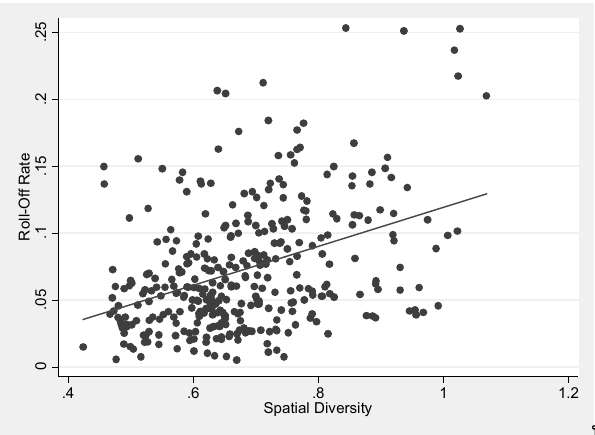
\includegraphics{img/sd_rolloff.png}
\caption{Effect of spatial diversity on electoral rolloff}
\end{figure}

\begin{figure}
\centering
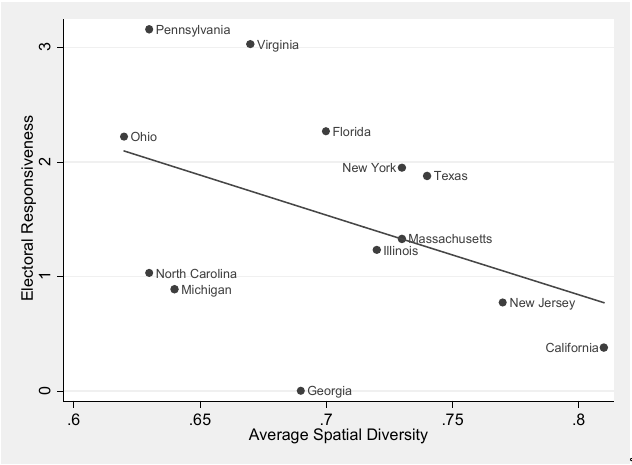
\includegraphics{./img/average_spatial-diversity.png}
\caption{Effect of electoral responsiveness on spatial diversity}
\end{figure}

\begin{quote}
spatial diversity remained a statistically significant predictor of
roll-off rate. With these variables held constant at their means, a
House district's shift from the tenth to the ninetieth percentile in
spatial diversity was associated with an increase in roll-off rate of
about six percentage points
\end{quote}

The final political gerrymandering issue that I investigate is how
spatial diversity relates to common dis- trict plan metrics such as
partisan bias and electoral responsiveness. As noted earlier, partisan
bias refers to the divergence in the share of seats that each party
would win given the same share of the statewide vote.254 For example, if
Democrats would win forty-eight percent of the seats with fifty percent
of the vote (in which case Republicans would win fifty-two percent of
the seats), then a district plan would have a pro-Republican bias of two
percent. Electoral responsiveness refers to the rate at which a party
gains or loses seats given changes in its statewide vote share. For
instance, if Democrats would win ten percent more seats if they received
five percent more of the vote, then a plan would have a responsiveness
of 2.0. 255 As a general matter, the lower a plan's bias, and the higher
its responsiveness, the better the plan is thought to be. 256

255 See Gelman \& King, supra note 11, at 544--45 (defining bias and
responsiveness). 256 Reducing bias all the way to zero is unproblematic.
However, very high rates of responsiveness are undesirable because they
result in large changes in seat shares despite only small shifts in vote
shares. Fortunately, the responsiveness scores reported here are not
high enough to raise such concerns.

Figures 12 and 13 show how states' spatial diversity averages were
related to partisan bias and electoral responsiveness in the 2006, 2008,
and 2010 elections.260 I include only states with at least ten congres-
sional districts (because bias and responsiveness are not very meaning-
ful for states with small numbers of seats), 261 and I use the absolute
value of bias (because I am interested in the metric's magnitude rather
than its orientation). As is evident from the first chart, spatial
diversi- ty has a curvilinear relationship with bias. At lower levels of
spatial diversity, that is, bias tends to decrease as spatial diversity
increases; but at higher levels of spatial diversity, bias and spatial
diversity tend to move in tandem. The curve as a whole is clearly
U-shaped. 262 This result suggests that states seeking to treat the
major parties as equitably as possible should not minimize the average
spatial diversity of their districts. Consistent with the relevant
literature, high levels of geographic variation are associated with high
bias; 263 they both imply

The story with responsiveness is more straightforward. As the se- cond
chart illustrates, responsiveness simply tends to decrease as aver- age
spatial diversity increases. The states whose districts are most
homogeneous, on average, are also the states whose elections are most
responsive to changes in public opinion. In contrast, the states whose
districts are most heterogeneous are also the ones in which even large
swings in voter sentiment have little impact on the parties' seat
shares. This finding indicates that while high spatial diversity is not
a prereq- uisite for a partisan gerrymander (low spatial diversity can
also do the trick), it is indeed an effective way to protect incumbents
of both par- ties from shifting political tides. Advocates of responsive
elections, then, may push without hesitation for spatially homogeneous
districts to be drawn, since it is these districts that seem most likely
(in the ag- gregate) to reflect the public's evolving preferences. 265

\cite{steph2012}

\hypertarget{how-compactness-might-affect-spatial-diversity}{%
\subsubsection{How compactness might affect spatial
diversity}\label{how-compactness-might-affect-spatial-diversity}}

\hypertarget{previous-work}{%
\subsubsection{Previous work}\label{previous-work}}

\begin{itemize}
\tightlist
\item
  people have done how compactness affects competitiveness (schutzman
  2020)
\item
  people have used MCMC approach to look at how districts are more or
  less competitive ( daryl's work)
\end{itemize}

\hypertarget{overview-of-research-strategy}{%
\subsection{Overview of research
strategy}\label{overview-of-research-strategy}}

Two key research questions:

\begin{enumerate}
\def\labelenumi{\arabic{enumi}.}
\tightlist
\item
  Do more compact districts have better, equal, or worse spatial
  diversity scores?
\item
  Is there an inherent trade-off between compactness and homogeneity?
\item
  Does spatial diversity give us a normative basis to select one
  compactness metric over another?
\end{enumerate}

The research procedure:

\begin{enumerate}
\def\labelenumi{\arabic{enumi}.}
\item
  Generate a large and representative subset of plausible districting
  plans
\item
\end{enumerate}

\hypertarget{overview-of-compactness-measures}{%
\subsubsection{Overview of compactness
measures}\label{overview-of-compactness-measures}}

To empirically evaluate a trade-off between compactness and homogeneity,
we must first define the metrics by which we evaluate a proposed
districting plan over each of these dimensions. Here, I introduce many
different compactness measures. I give a brief overview of the different
types of measures, explain the pros and cons of each, present a
compactness measure that I develop, and support my decision to use an
ensemble of measures to increase robustness.

\hypertarget{geometric-compactness-metrics}{%
\paragraph{Geometric compactness
metrics}\label{geometric-compactness-metrics}}

Shape-based versus dispersion-based

The most

\hypertarget{polsby-popper}{%
\paragraph{Polsby-Popper}\label{polsby-popper}}

The Polsby-Popper measure, introduced by Polsby and Popper in 1991, is a
ratio of the area of the district to the area of a circle whose
circumference is equal to the perimeter of the district.

\[4\pi \times \frac{A}{P^2}\]

\begin{figure}
\centering
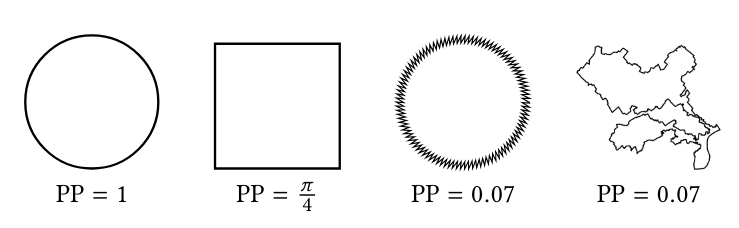
\includegraphics{img/pp_example.png}
\caption{Polsby-Popper scores of four example regions: a perfect circle,
a square, a circle with a ragged boundary, an an example district from a
Pennsylvania plan. Taken from \cite{s2020}.}
\end{figure}

\hypertarget{reock}{%
\paragraph{Reock}\label{reock}}

The Reock score is a measure of the ratio of the district to the area of
the minimum bounding circle that encloses the district's geometry.

\[\frac{Area}{AreaOfMinimumBoundingCircle}\]

\hypertarget{convex-hull}{%
\paragraph{Convex Hull}\label{convex-hull}}

The Convex Hull metric is a ratio of the area of the district to the
area of the minimum convex polygon that can enclose the district's
geometry.

\[\frac{Area}{AreaOfMinimumConvexPolygon}\]

\hypertarget{choosing-a-compactness-metric}{%
\paragraph{Choosing a compactness
metric}\label{choosing-a-compactness-metric}}

Which compactness measure should we choose? All three compactness
measures are well-cited in the literature and enjoy widespread use. They
have been cited in U.S. Supreme Court cases, \emph{amici} briefs, and
redistricting commissions \citep{moncrief2011}. Despite their widespread
acceptance, however, the problems with compactness measures are many,
and well-covered in the literature. No compactness measure is perfect:
as an example, the most popular compactness measure in the
literature---Polsby-Popper---is sensitive to small perturbations in data
resolution (the coastline problem). \footnote{The Polsby-Popper metric
  measures the ratio of the area of the district to the area of a circle
  whose circumference is equal to the perimeter of the district. But
  depending on the resolution of the map, the perimeter can be
  effectively infinite. \citeauthor{bswp} find that the choice of
  resolution has ``a substantial impact on compactness scores, with the
  Polsby-Popper score especially affected.''} It is therefore important
to use an \emph{ensemble} of compactness measures to make sure that
one's data and conclusions are robust.

But even this is not enough. Because most compactness measures are
purely geometric, they are all vulnerable to a specific family of
geographic perturbations. Indeed, \cite{bswp} show that minimally
tweaking the geometric features of states is enough for the four most
popular compactness measures (Polsby-Popper, Convex Hull, Reock,
Schwartzberg) to give very different conclusions on nominally identical
data.

Thus, it is important to include a non-geometric compactness measure in
the ensemble to guard against the possibility that the results are
driven by a specific quirk in geography. Many such measures have been
proposed. For instance, \cite{dc2016} bring in a discipline of
mathematics---graph theory---to formulate a new metric of compactness.

However, one particular class of metrics I term \emph{point-wise
distance metrics} stands out for its ease of understanding (critical if
it is to be persuasive to Supreme Court judges), theoretical
attractiveness, and academic consensus. This class of compactness
metrics tries to measure the distance between two voters in a district,
and assigns higher scores the lower that distance is.

This class of metrics enjoy strong theoretical grounding. Paramount to
the idea of single-member districts is that there is some value in
voters who live in the same area being put into the same district.
\cite{er2019}:

\begin{quote}
``Voters in the same area are likely to share political interests;
voters in the same area are better able to communicate and coordinate
with one another; politicians can better maintain connections with
voters in the same area; voters in the same area are especially likely
to belong to the same social communities --- all suggest the importance
of voters being located in districts with their geographic peers.''
\end{quote}

In contrast, districts that carve voters out of their natural
communities and pool them with unrelated, distant voters are bad ones.
Therefore, we should be sensitive not just to geometric shape, but
rather whether or not voters live close to one another. Point-wise
distance metrics are more readily understandable to laymen and possess a
normative bent that more abstract mathematical compactness measures
lack. It has therefore been an active area of development in the
literature. \cite{cm2010} present a measure of ``bizarreness'', which is
the ``expected relative difficulty in traveling between two points
within the district''. And \cite{fh2011} measures ``the distance between
voters within the same district relative to the minimum distance
achievable''.

I build upon the literature by developing a new metric which I call
human compactness. The metric measures the ratio of driving durations
between one's nearest neighbours and one's fellow districtors. The
higher this ratio is, the more compact the district. Intuitively, it
encourages drawing districts that put one's next-door neighbours
together in the same district. This metric makes two key improvements
over existing measures that have been proposed.

\textbf{TODO explain my metric a bit more before talking about the
improvements Maybe change tack --- criticise the existing literature
approach/ talk about shortcomings, then introduce my metric.}

First, I use driving durations rather than Euclidean (as-the-crow-flies)
distances between voters. This keeps the metric robust to quirks in
political geography like mountains and lakes, and better represents the
notion of natural communities. In fact, while \cite{fh2011} used
Euclidean distance in his metric, he points out its shortcomings:

\begin{quote}
Suppose there is a city on a hill. On the West side is {[}a{]} mild,
long incline toward the rest of the city, which is in a plane. On the
East side is a steep cliff, either impassable or with just a narrow,
winding road that very few people use. While the next residential center
to the East is much closer to the hilltop on a horizontal plane, it is
much further on all sorts of distances that we think might matter:
transportation time, intensity of social interactions, sets of shared
local public goods and common interests, etc. Thus, for all practical
purposes, one probably wants to include the hilltop in a Western
district rather than an Eastern one. More general notions of distance
can handle this.
\end{quote}

In this case, driving durations would better reflect this quirk in
political geography. The ``impassable'' region on the East would have a
short Euclidean distance, and any districting plan that put the hilltop
with the Eastern district would be unfairly penalised by these
point-wise distance metrics. On the other hand, the impassable region
would have a long driving duration, accurately reflecting the political
geography. After acknowledging the shortcomings of Euclidean distance,
\citeauthor{fh2011} specifically suggest using driving durations to
improve their metric: ``one can extend much of {[}our analysis{]} by
using driving distance or what legal scholars refer to as `communities
of interest'\,''.

There are thus strong theoretical grounds for using driving durations in
point-wise distance metrics. Driving durations also enjoys empirical
support---the use of driving durations seems strictly superior in many
cases involving human-scale distances. Working with Nicholas Eubank and
Jonathan Rodden, I update their gerrymandering-detection metric to use
driving durations instead \citep{er2019}. We find a consistently
different picture of the social context of American suburban voters,
raising the possibility of false positives under the Euclidean distance
measure \citep*{elrwp}.

The second improvement I make is algorithmic and computational. My
metric improves upon the algorithmic complexity of \citeauthor{fh2011}'s
algorithm from an NP-hard problem to one with a \(O(n^2)\) polynomial
runtime. This is an exponential decrease in algorithmic complexity,
which means the disparity between my metric and \citeauthor{fh2011}'s
increases as the input size grows. Similarly, \citeauthor{cm2010}'s
measure cannot feasibly be improved with driving durations due to the
algorithmic complexity of finding point-to-point travel distances
without passing through another district \footnote{The metric uses the
  probability that the shortest path between any two points in the
  district is exactly the shortest path between any two points in the
  state. This requires finding the shortest path between all points in
  the district subgraph, which has O(n\^{}3) complexity in the best
  case, but in practice has a larger complexity because we are querying
  a routing engine for travel times.}. Given that there are strong
theoretical and empirical reasons to adopt driving durations, this is a
large improvement. I also use programming techniques like precomputation
and memoisation to decrease the time taken to compute the metric
greatly. My implementation is competitive with geometry-based
compactness measures like Reock: on my machine, both metrics took
roughly the same amount of time (\textasciitilde{}0.20s per step).
Further details on the metric can be found in Appendix A.

Given these considerations, I settle on an ensemble of four different
compactness measures: Polsby-Popper, Reock, Convex Hull, and Human
Compactness. I exclude the Schwartzberg metric as the Schwartzberg and
Polsby-Popper measure are mathematically equivalent. Finally, I include
my point-wise distance metric. This ensures the robustness and validity
of my results.

\hypertarget{overview-of-automated-districting-algorithms}{%
\subsubsection{Overview of automated districting
algorithms}\label{overview-of-automated-districting-algorithms}}

In order to find out whether compactness measures track spatial
diversity, we have to generate many counterfactual plausible plans that
span the entirety of possible districting plans and measure the
correlation between compactness and spatial diversity. This requires
using a computer to draw a large number of plans according to some
minimal criteria.

The idea of drawing a large number of districting plans with a computer
has a long and storied history, starting in the 60s and 70s. The
approach has almost always been used to identify gerrymandering; for
instance \cite{ccd2000} build an algorithm to ``quantitatively
{[}assess{]} whether the {[}1990 South Carolina{]} plan is a racial
gerrymander''. More recently, \cite{cr2013} ``generat{[}e{]} a large
number of hypothetical alternative districting plans that are blind as
to party and race, relying only on criteria of geographic contiguity and
compactness.'' They do this using a Markov Chain simulation algorithm, a
procedure that makes iterative changes for a large number of steps until
a unique districting plan emerges. At each step of
\citeauthor{ccd2000}'s algorithm, they randomly select a Census Block
Group to serve as a ``seed'' of the district, then randomly add its
neighbouring block groups to it until a district with the desired
population is formed. Similarly, \citeauthor{cr2013} begin by
initialising all precincts as an individual, separate district, then
randomly agglomerating neighbouring precincts until the desired number
of districts is reached.

While this ``standard simulation algorithm'' enjoys a certain degree of
success, it has one crippling weakness. The way in which this class of
algorithms operates necessarily explores only a tiny subset of all
possible districting plans. Subsequent work pointed out this flaw:
\citeauthor{mm2018} wrote that automated processes ``may take a biased
sample of all possible legislative maps\ldots{} and fail to efficiently
produce a meaningful distribution of all alternative maps''. And
\citeauthor{fifieldwp} contend that ``{[}standard Monte Carlo
algorithms{]} are unlikely to yield a representative sample of
redistricting plans for a target population.'' \footnote{See
  \cite{fifieldwp}, pg. 16, for a technical explanation of why these
  algorithms don't produce uniform redistricting plans: ``For example
  \ldots{}, the creation of earlier districts may make it impossible to
  yield contiguous districts. These algorithms rely on rejection
  sampling to incorporate constraints, which is an inefficient strategy.
  More importantly, the algorithms come with no theoretical result and
  are not even designed to uniformly sample redistricting plans.''} This
poses a huge issue for the validity of any statistical analysis, because
any correlation that we discover on a biased subset of plans may be
spurious when measured over the actual distribution of plans. \footnote{Generating
  a biased sample is not necessarily a problem if all you want to do is
  \emph{optimise}, e.g.~draw the most compact plan possible. Recent work
  builds upon this standard algorithm, using Voronoi diagrams or
  iterative flood fill procedures rather than random chance, to assign
  the precincts to be agglomerated. See \cite{lf2019} for a technical
  overview.}

Thankfully, scholars have developed an improvement over the standard
algorithm with stronger theoretical guarantees. This second class of
algorithms reframe the districting problem as a \emph{graph partition}
problem (borrowing insights from graph theory and computer science), and
use a \emph{Markov Chain Monte Carlo} (MCMC) approach to sample possible
districting plans. This approach is best laid out in \cite{fifieldwp}.
Broadly speaking, the approach initialises a specific graph partition as
a step in the Markov Chain, then \emph{flips} a random node of the graph
to get another valid partition. This process is repeated until the
Markov Chain approaches its steady state distribution: when this
happens, the Markov chain is called ``well-mixed''.

This class of algorithms inherit desirable well-known theoretical
guarantees of the Markov Chain.\footnote{See \cite{ddj2019recom} for a
  technical overview.} They are therefore much less likely (both
theoretically and empirically) to generate a biased subset of plans.
Conducting a small-scale validation study on a 25-precinct set,
\citeauthor{fifieldwp} compare the distribution of plans generated by
their algorithm to those generated by the standard redistricting
algorithm. They prove that their algorithm produces plans that hew much
more closely to the \emph{actual} distribution of all possible
districting plans.

Due to the many advantages of the MCMC approach, I use it in all my
analyses. I use an superior proposal distribution called Recombination
(Recom) by \citeauthor{ddj2019recom}, which uses a spanning tree method
to bipartition pairs of adjacent districts at each step
\citep{ddj2019comp}. This proposal distribution improves upon the
\texttt{Flip} proposal in \citeauthor{fifieldwp} in two significant
ways: it generates plans in much fewer steps \footnote{the ``mixing
  time'' of the Markov Chain---that is, the number of steps it takes for
  the Markov Chain to be ``close enough'' to the stationary
  distribution---is order of magnitudes smaller in \texttt{Recom}
  compared to \texttt{Flip}.}, and it generates plans that are much more
realistic. The \texttt{Flip} proposal tends to generate very uncompact,
snakelike districts, as can be seen in the figure.

\begin{figure}
\centering
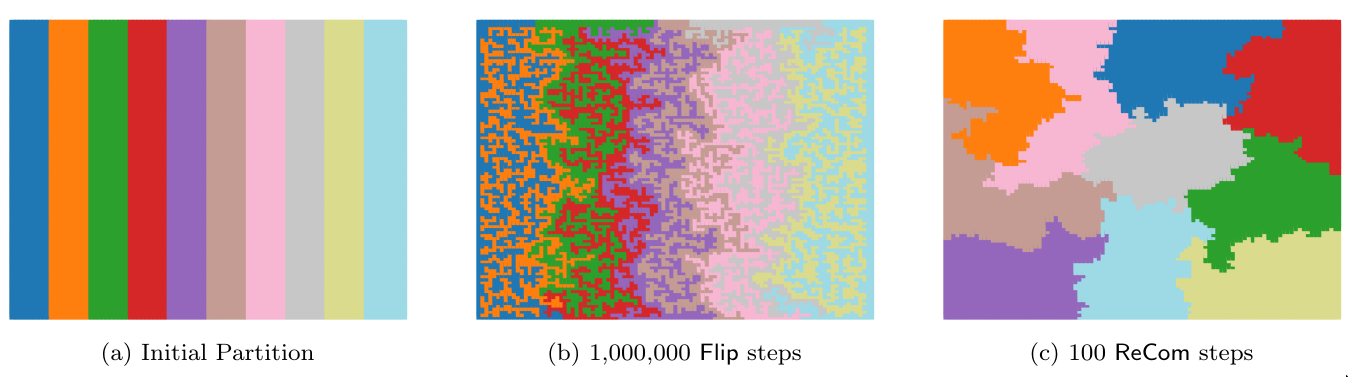
\includegraphics{img/recom_vs_flip.png}
\caption{The \texttt{Recom} proposal generates more realistic plans in
much fewer steps. Taken from \cite{ddj2019recom}.}
\end{figure}

\hypertarget{data-generation}{%
\subsection{Data generation}\label{data-generation}}

\begin{enumerate}
\def\labelenumi{\arabic{enumi}.}
\tightlist
\item
  Generate 100,000 districting plans
\end{enumerate}

I download Census Tract level. These can be downloaded from the
\href{census.gov}{United States Census Bureau} website.

I use the open-source software library GerryChain to generate the
ensembles. Replication code and data are included in the Supplementary
Information. I obtain the ReCom Markov chain procedure from one of the
co-authors of the \cite{ddj2019recom} paper, and generate 10,000
districting plans for 10 states (Connecticut, Georgia, Idaho, Louisiana,
Maine, Maryland, New Hampshire, Rhode Island, Utah, and Wisconsin) for a
total of 100,000 plans.

\begin{enumerate}
\def\labelenumi{\arabic{enumi}.}
\setcounter{enumi}{1}
\tightlist
\item
  Calculate spatial diversity and compactness scores for each of the
  100,000 districting plans
\end{enumerate}

I obtain data on spatial diversity from Professor Nicholas
Stephanopoulos. The dataset gives \emph{factor scores} for each Census
Tract in the country. A district's spatial diversity score is calculated
by the sum of the standard deviation of each factor score, normalised by
the proportion of the variance each factor score explains. As an
example, consider a district made up of three Census Tracts (A, B, C)
and let each Tract have three factor scores (1, 2, 3). Let the
proportion of the variance explained by each factor score be 50\%, 30\%
and 20\% respectively. Then the total spatial diversity score would be

\[ \sigma(A_1, B_1, C_1) \times 0.5 + \sigma(A_2, B_2, C_2) \times 0.3 + \sigma(A_3,
B_3, C_3) \times 0.2\]

Because

I obtain voter data from \citeauthor{er2019},

In order to do this, I have to

\begin{enumerate}
\def\labelenumi{\arabic{enumi}.}
\setcounter{enumi}{2}
\tightlist
\item
  Analyse
\end{enumerate}

As a robustness check, I rerun all the analyses

by taking the sum of square roots rather than the arithmetic mean.

This penalises districting plans that have a large difference between
districts e.g.~one very good district and one very bad one.

\hypertarget{results}{%
\subsection{Results}\label{results}}

My key results are as follows:

\begin{enumerate}
\def\labelenumi{\arabic{enumi}.}
\tightlist
\item
  Political geography largely pins down the spatial diversity of each
  individual district.

  \begin{itemize}
  \tightlist
  \item
    Small urban districts have high SD, large rural ones have low SD.
  \end{itemize}
\item
  Different compactness measures are correlated with one another.
\item
  OLS regressions and difference-in-means tests suggest that only the
  human compactness measure is negatively correlated with spatial
  diversity: geometric/dispersion based measures have either no or a
  positive (bad) effect on spatial diversity.
\item
  A difference-in-means test suggests that the most compact districting
  plans are indeed less spatially diverse than average.
\item
  A difference-in-means test suggests that the most compact plans under
  human compactness are less spatially diverse than the most compact
  plans under geometric/dispersion based measures.
\end{enumerate}

Overall, the evidence suggests that optimising over compactness will
give you less spatially diverse districts, and human compactness will do
the best job of it.

\hypertarget{descriptive-analysis}{%
\subsubsection{Descriptive analysis}\label{descriptive-analysis}}

After having obtained all the plans and their corresponding scores, I
plot the plans with the best and worst spatial diversity and compactness
scores to get an understanding for the types of plans that each metric
encourages. This will give us valuable intuition for understanding the
subsequent results.

For ease of exposition we consider states with only two districts, but
the analysis extends to states with any number of districts. I also use
Polsby-Popper to represent the other two dispersion-based compactness
metrics as my explanations are similarly applicable to those metrics.

\begin{figure}
\centering
\includegraphics{../30_results/33_min_max_subplots.png}
\caption{Best and worst districting plans of New Hampshire under
different metrics \label{nh_minmax}}
\end{figure}

\begin{figure}
\centering
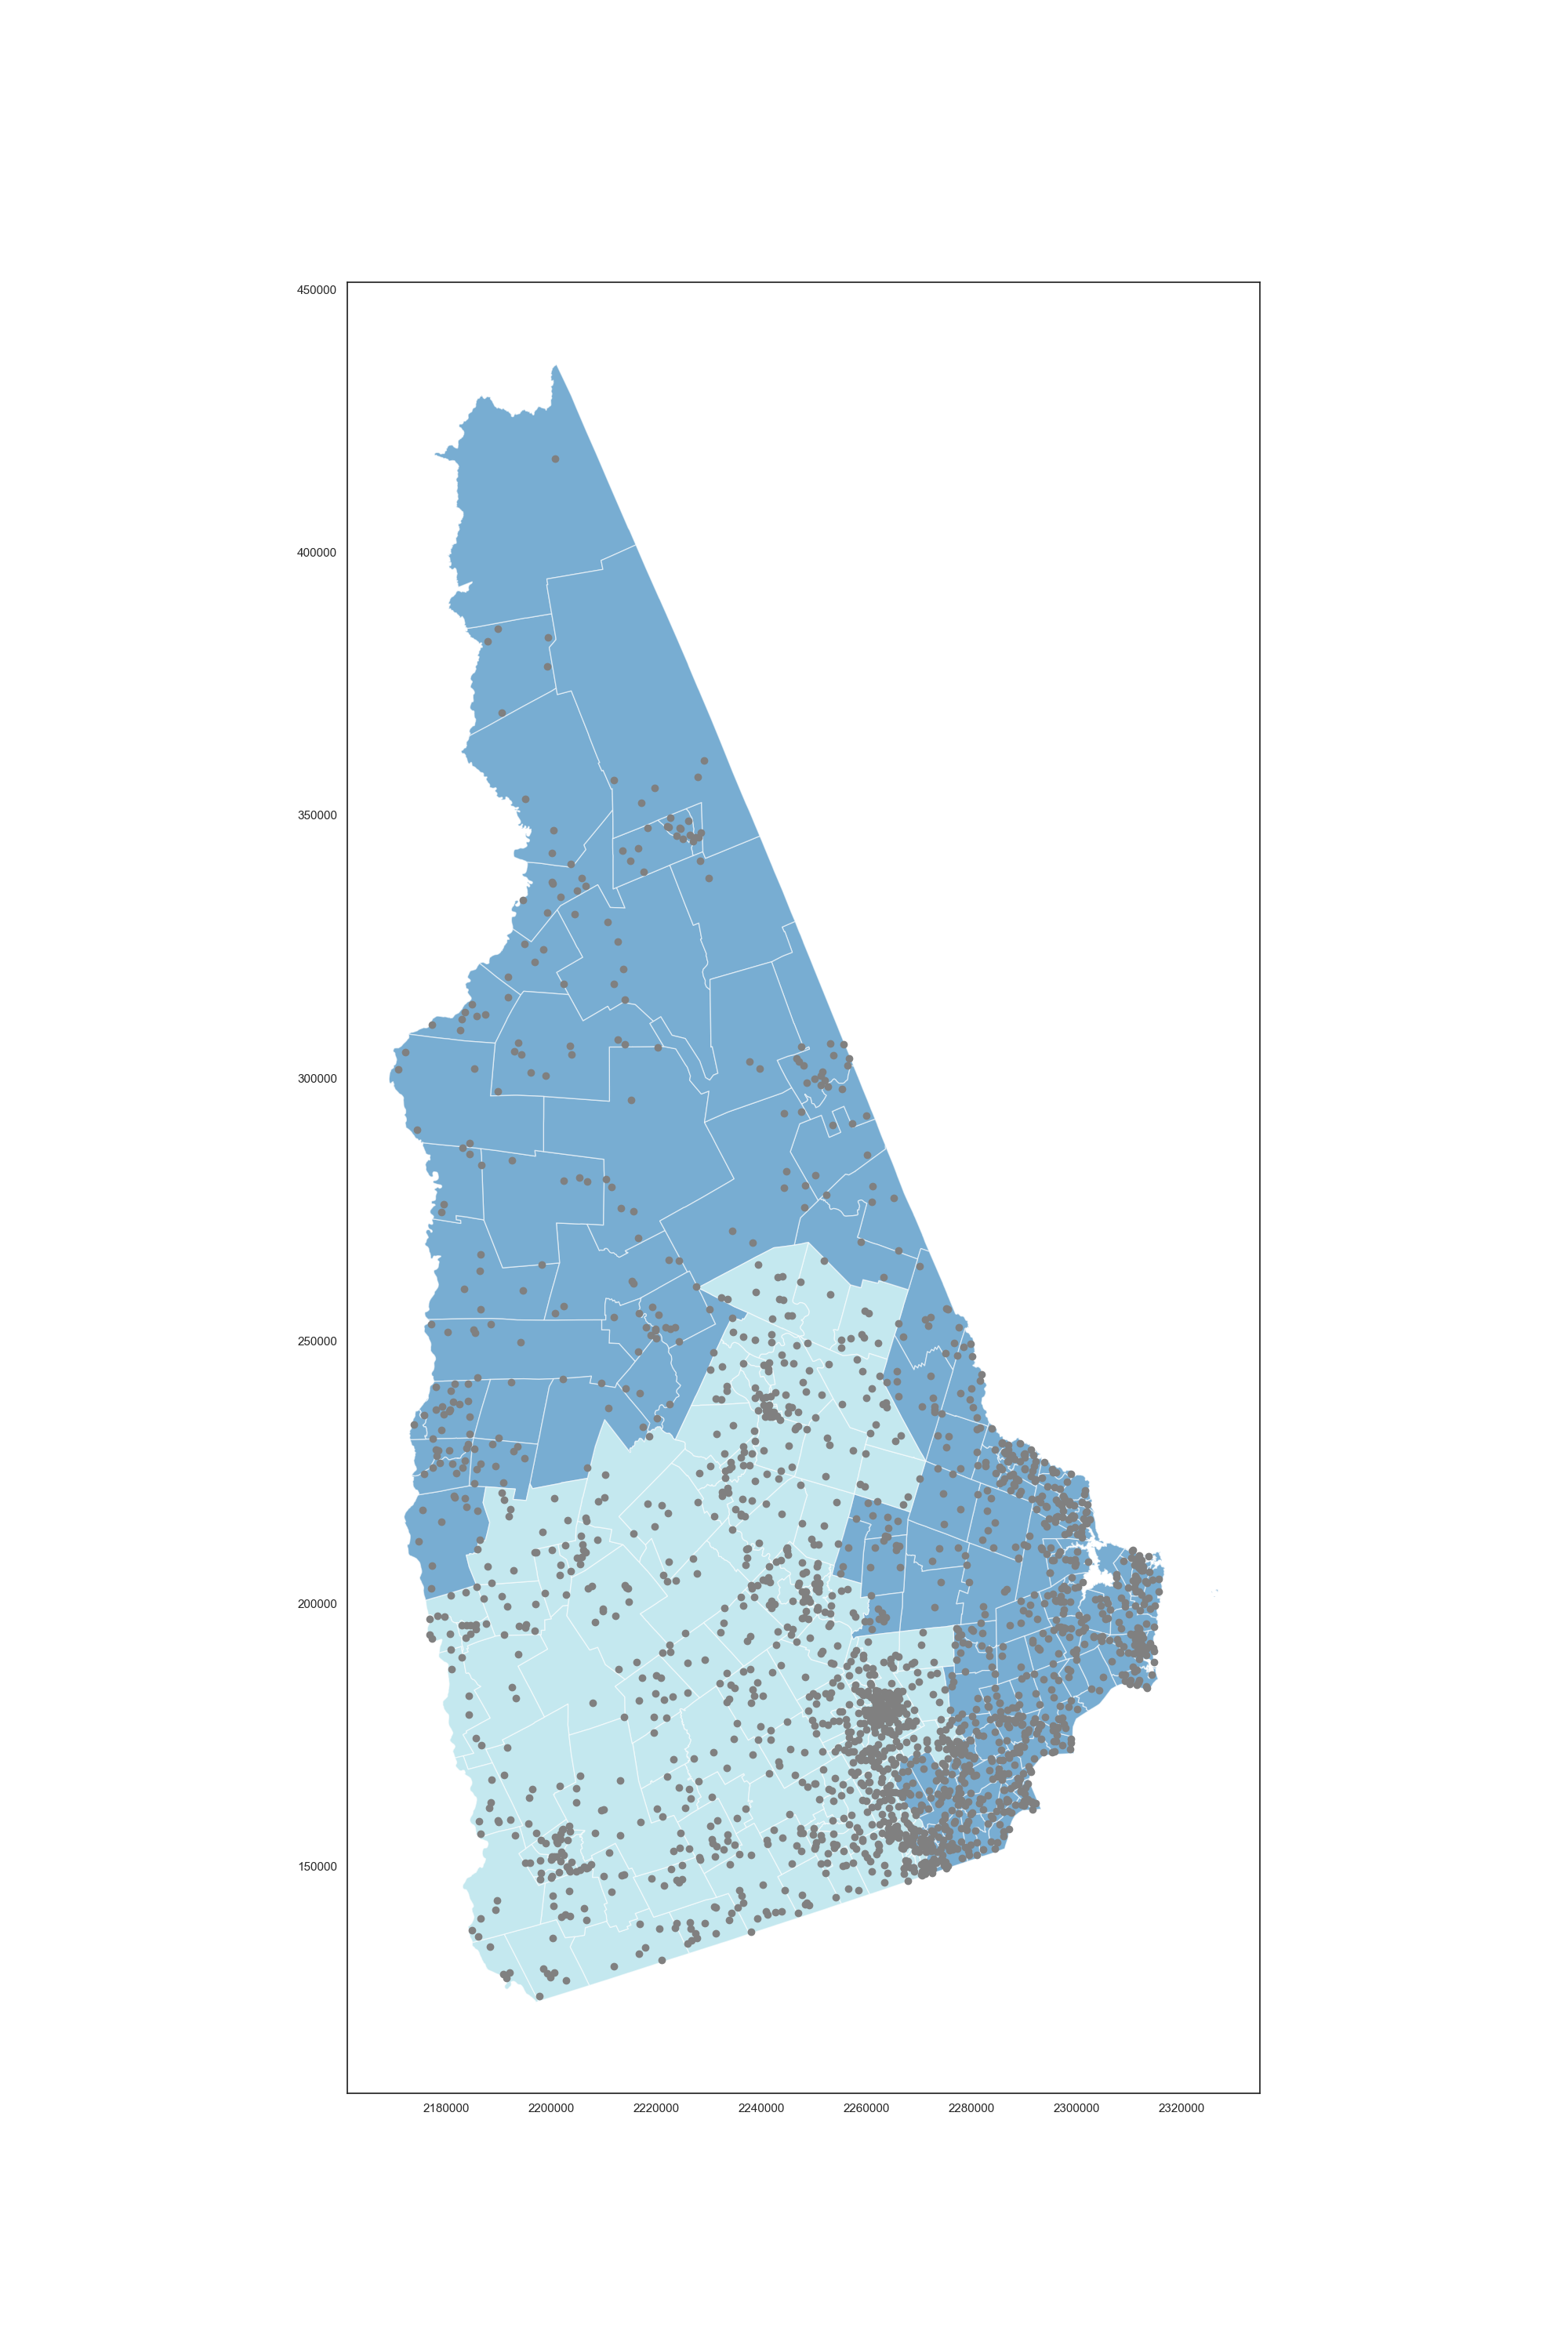
\includegraphics{../30_results/33_points_on_tracts.png}
\caption{Population density plot of New Hampshire. Each dot represents
roughly 600 people. \label{nh_density}}
\end{figure}

Figure \ref{nh_minmax} plots the best and worst plans according to
several metrics. Let us begin with the middle row (Polsby-Popper), as
its interpretation is the most straightforward. The Polsby-Popper (and
other dispersion-based) metric penalises districts that are very
``snakelike'' and prefers districts that have regular shapes like
squares or circles. This is clearly reflected in the plot. The best plan
has a district with a very regular shape, and the worst plan has a
snakelike district that contorts through half the state.

On the top row is human compactness. A good plan under human compactness
minimises the total travel times between every member of the district.
This encourages small, compact districts that avoid splitting urban
centers.

We can see that the top plan under human compactness corresponds well to
the actual population density of New Hampshire as seen in Figure
\ref{nh_density}. The top plan puts the two most populous and urban
counties in New Hampshire---Rockingham and Hillsborough---together in
the same district. The worst plan under human compactness splits the
counties in such a way that one's co-districtors are far away, and one's
nearest neighbours are in a separate district.

As expected, the top plan under spatial diversity (bottom row) closely
resembles the top plan under human compactness. In relatively
homogeneous New Hampshire, the main source of spatial diversity is the
urban-rural divide. A plan that keeps urbanites together in one district
is favoured under spatial diversity.

And while the worst plan under spatial diversity looks different from
that under human compactness at first glance, they are actually quite
similar. Both plans split up the two populous urban counties, having a
``fish-hook'' shaped district that starts from the rural north of the
state and swoops down to the south to carve out a large part of the
counties.

This case study shows that dispersion-based measures may not always
reflect existing communities of interest. This seems to fuel criticism
of dispersion-based measures on exactly that basis (``it makes no sense
to combine areas that have nothing in common except that they fit neatly
into a square'' \citep{wolf2015}). In this example, human compactness
and spatial diversity agree neatly on what the best districting plans
should look like.

While human compactness generally tracks spatial diversity better than
other compactness metrics (I provide evidence for this later), it does
not always do so.

\begin{figure}
\centering
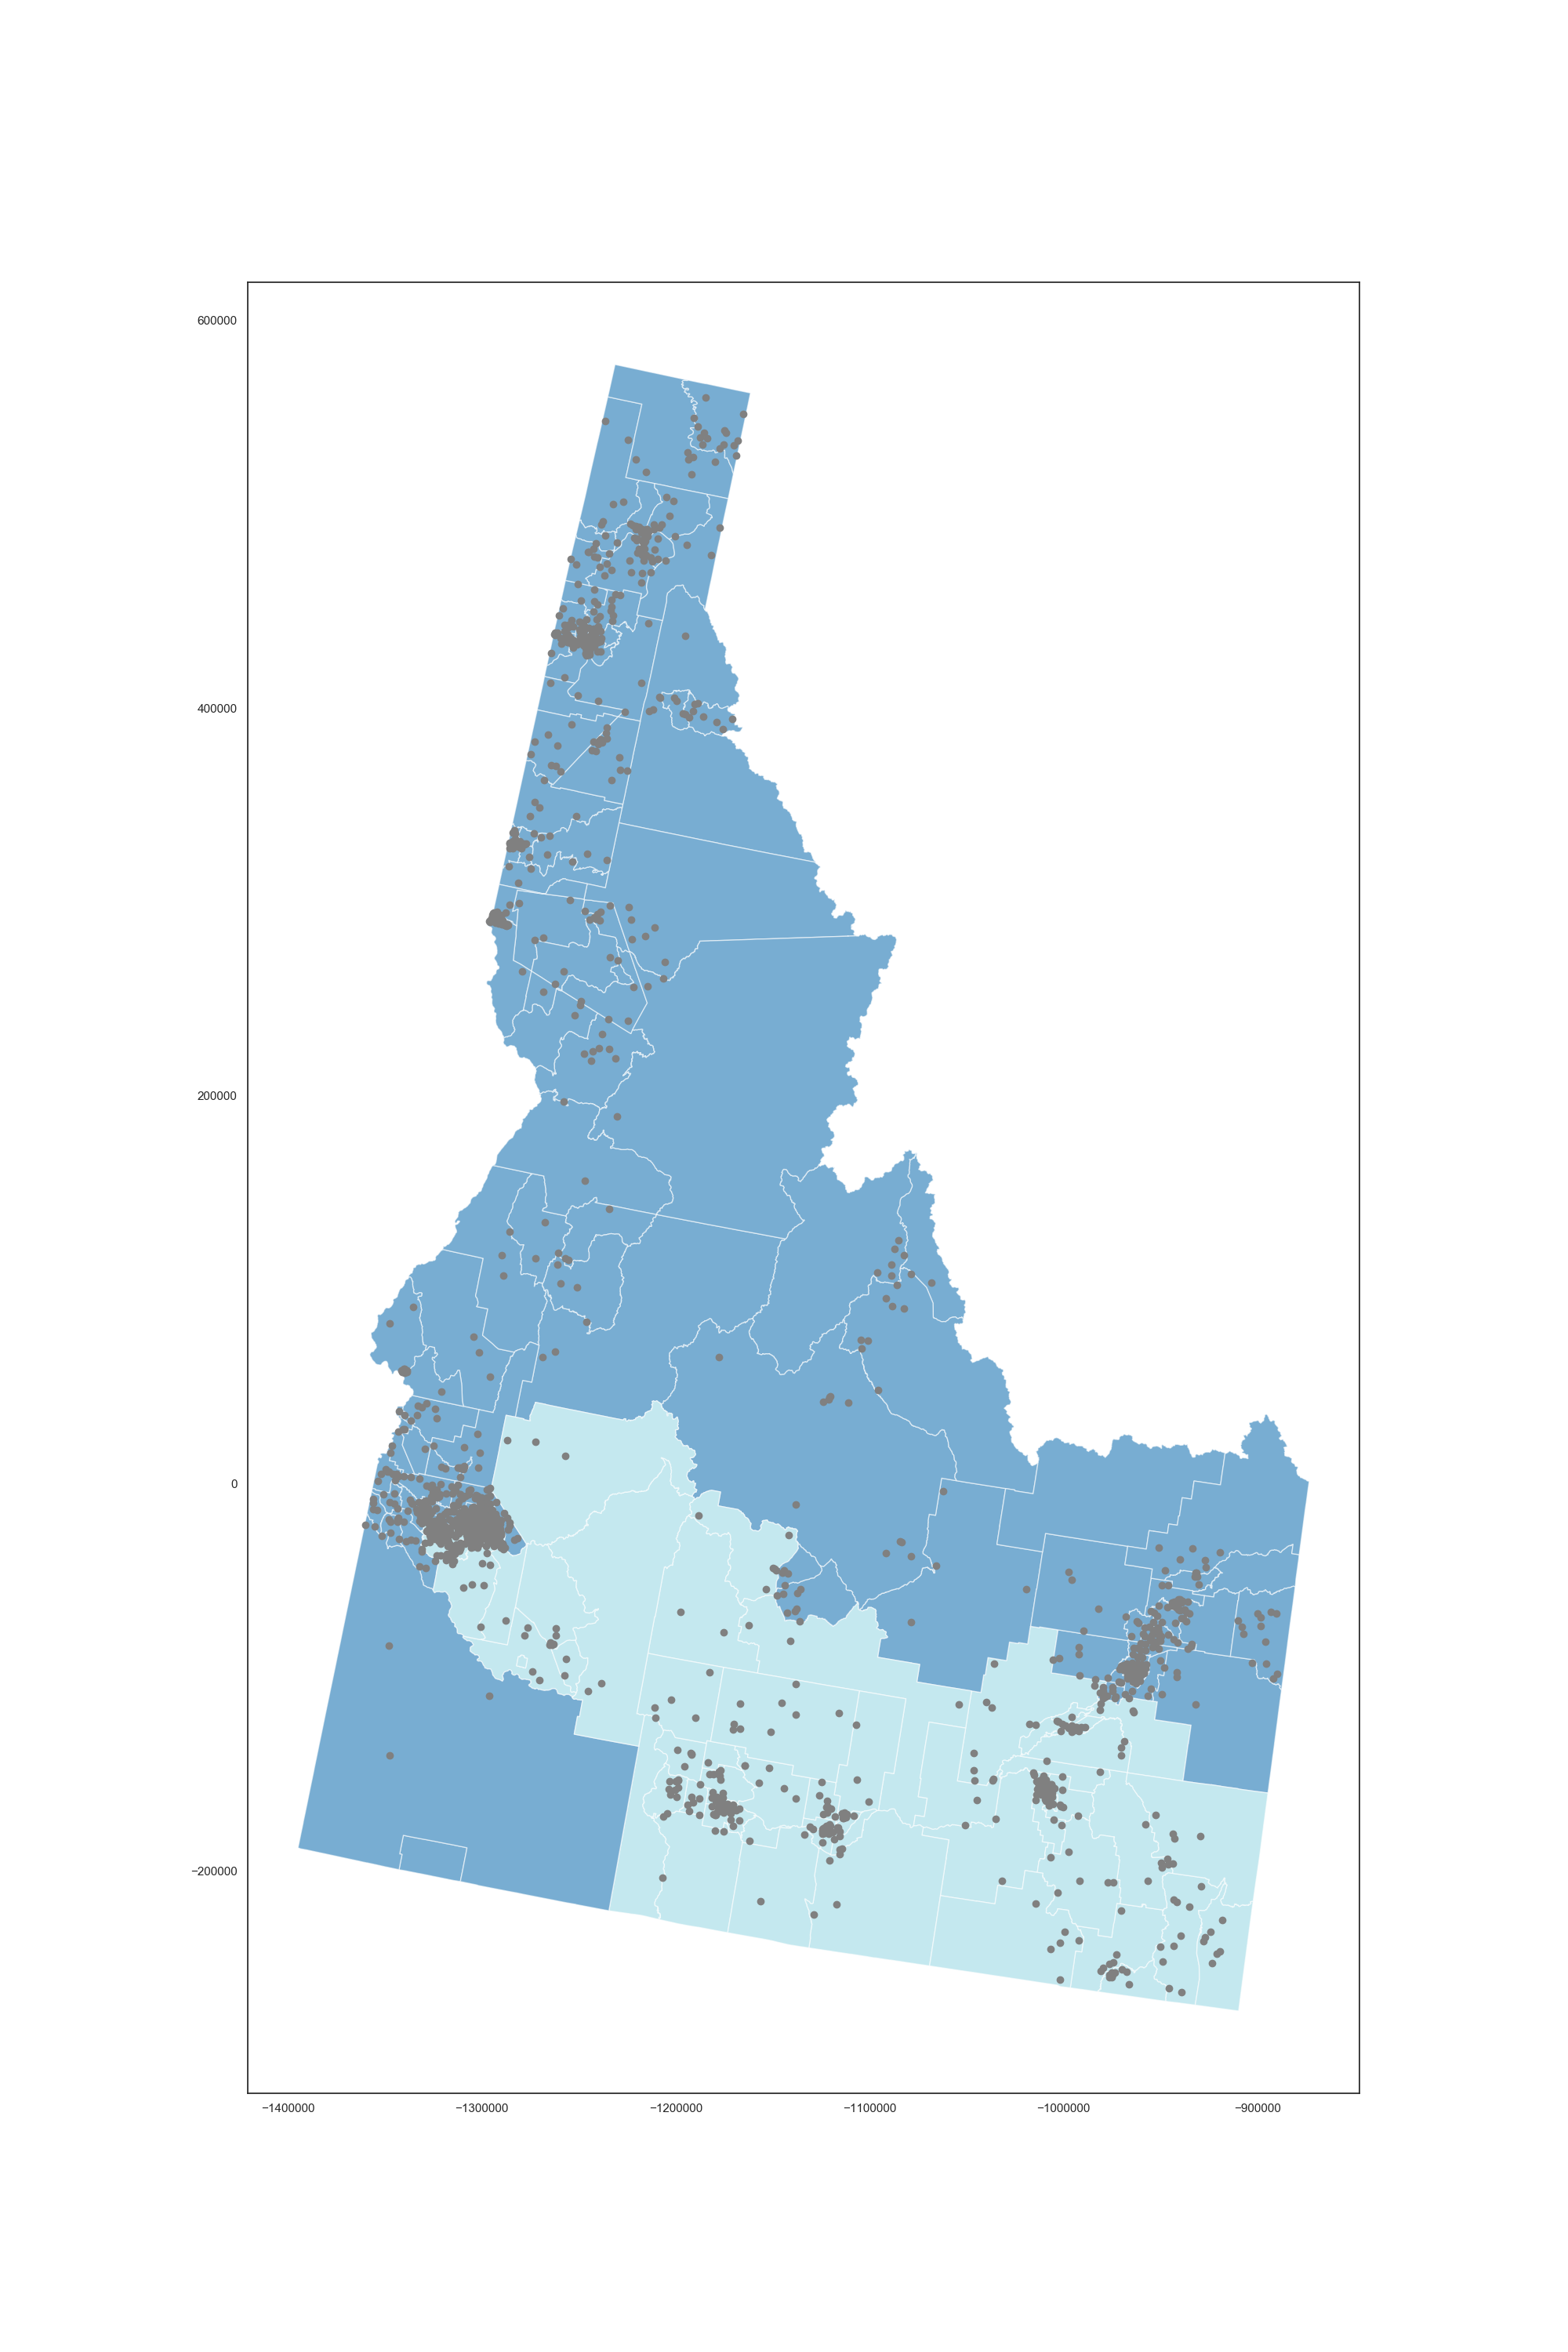
\includegraphics{../30_results/16_points_on_tracts.png}
\caption{Population density plot of Idaho. Each point represents
\textasciitilde{}700 people. \label{idaho_density}}
\end{figure}

\begin{figure}
\centering
\includegraphics{../30_results/16_min_max_subplots.png}
\caption{Best and worst districting plans of Idaho under different
metrics \label{idaho_minmax}}
\end{figure}

\hypertarget{political-geography-largely-pins-down-the-spatial-diversity-of-each-individual-district}{%
\subsubsection{Political geography largely pins down the spatial
diversity of each individual
district}\label{political-geography-largely-pins-down-the-spatial-diversity-of-each-individual-district}}

While spatial diversity varies enormously between districts, this is to
a large extent dependent on the state's political geography.

\begin{figure}
\centering
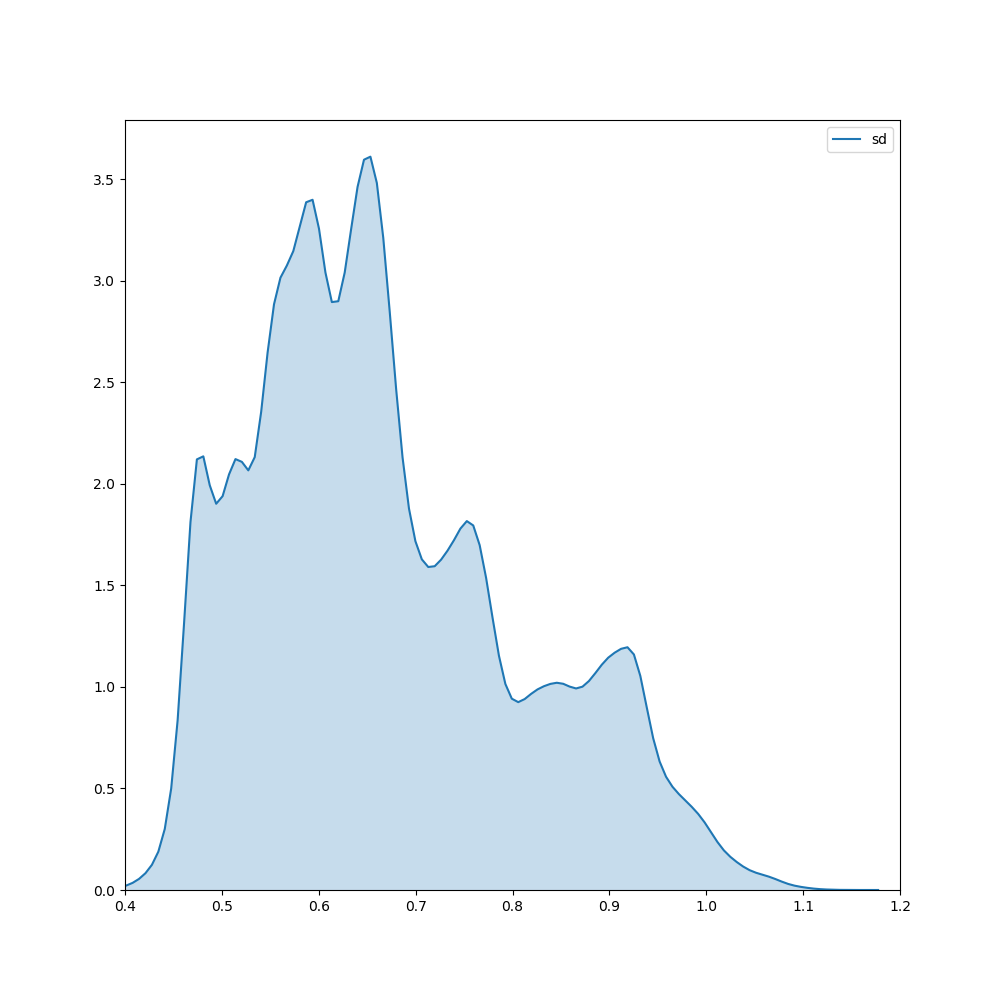
\includegraphics{../30_results/all_districts_concat_sd.png}
\caption{Spatial diversity of all districts}
\end{figure}

However, plotting individual states reveals great homogeneity.

\begin{figure}
\centering
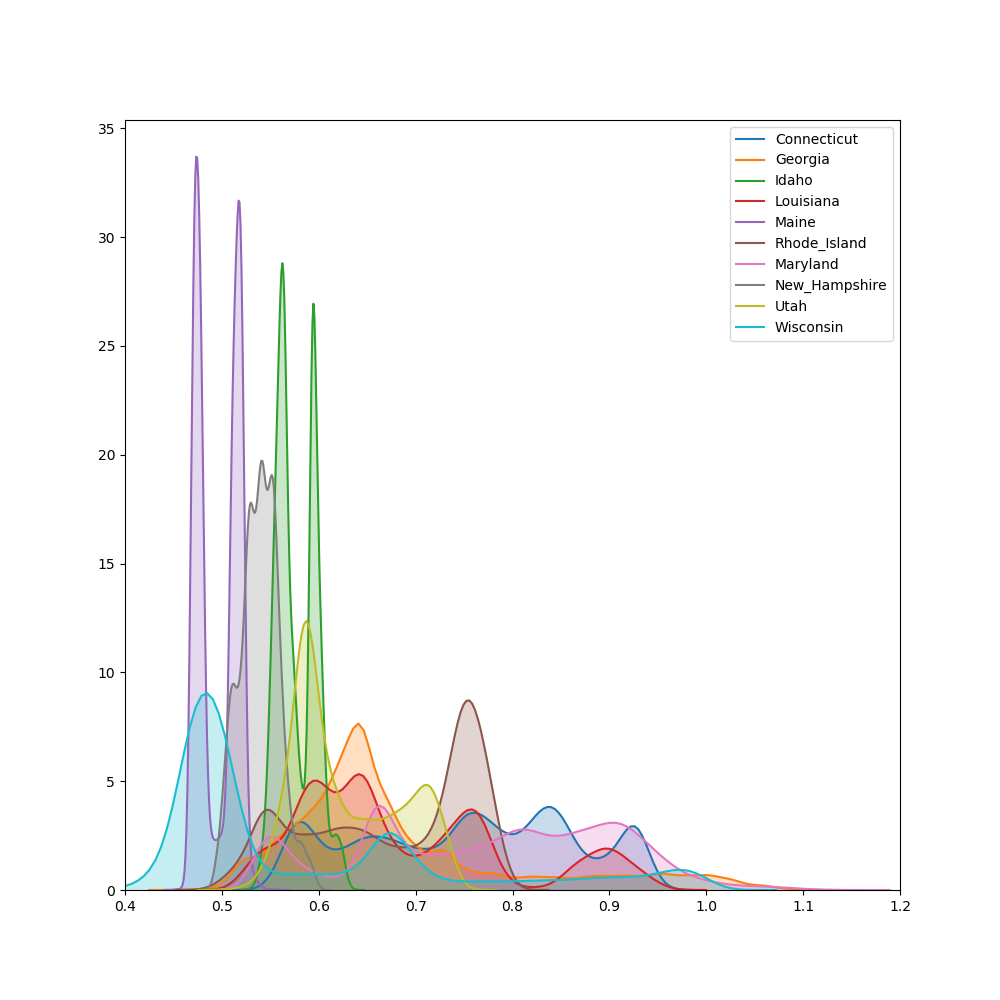
\includegraphics{../30_results/all_districts_sd.png}
\caption{Spatial diversity of districts binned by state}
\end{figure}

\begin{figure}
\centering
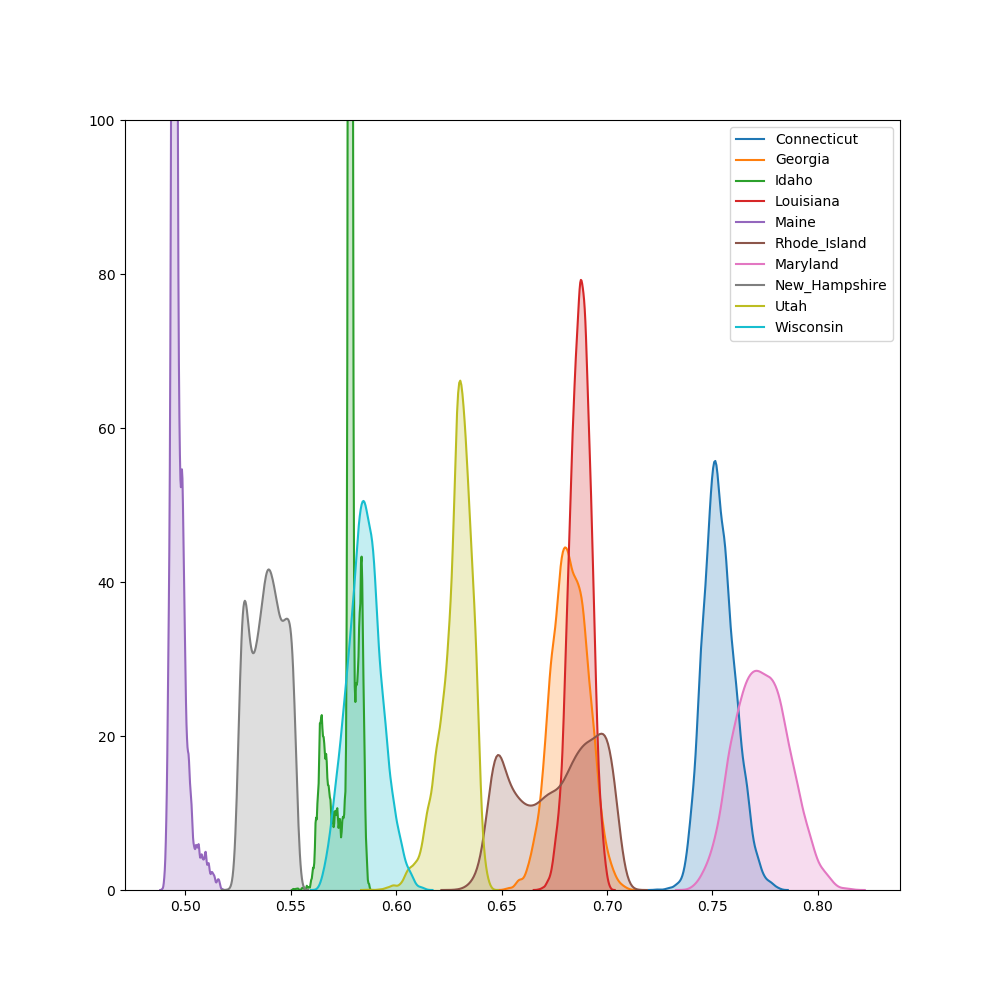
\includegraphics{../30_results/all_plans_sd.png}
\caption{Overall spatial diversity of districting plans by state}
\end{figure}

\hypertarget{compactness-measures-largely-agree-with-one-another-although-an-ensemble-is-still-required-due-to-possibility-of-outliers-actually-occurs}{%
\subsubsection{Compactness measures largely agree with one another,
although an ensemble is still required due to possibility of outliers
(actually
occurs)}\label{compactness-measures-largely-agree-with-one-another-although-an-ensemble-is-still-required-due-to-possibility-of-outliers-actually-occurs}}

\begin{verbatim}
             sd        hc        pp     reock        ch
sd     1.000000 -0.357926 -0.094629 -0.007729 -0.455142
hc    -0.357926  1.000000 -0.409995 -0.111860  0.110439
pp    -0.094629 -0.409995  1.000000  0.480940  0.606623
reock -0.007729 -0.111860  0.480940  1.000000  0.629797
ch    -0.455142  0.110439  0.606623  0.629797  1.000000
\end{verbatim}

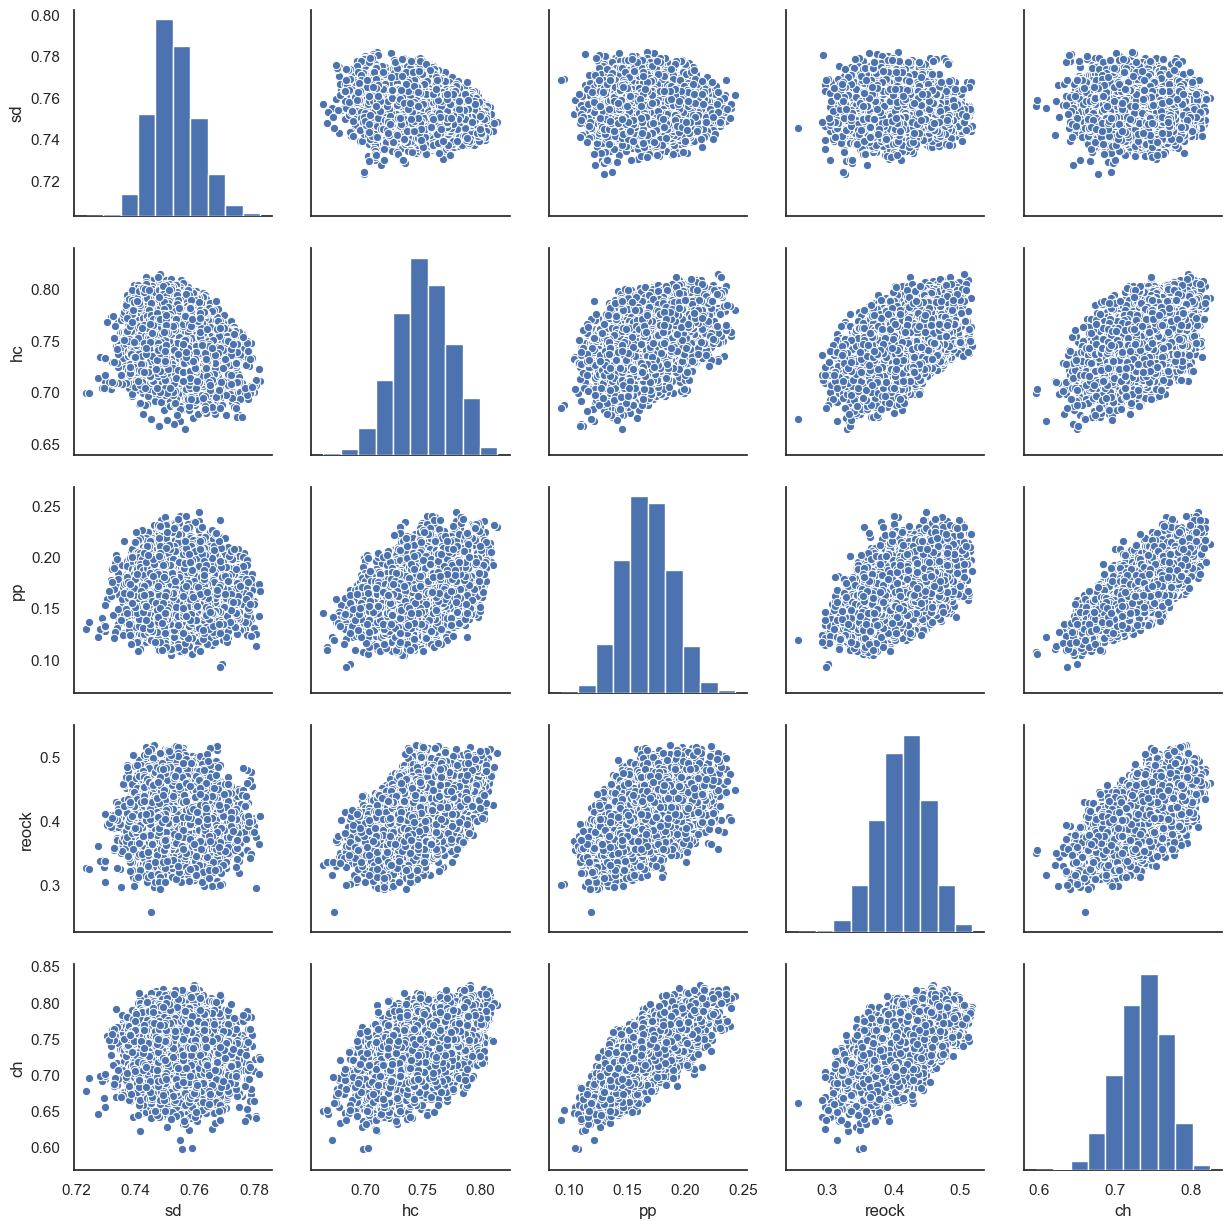
\includegraphics{../30_results/09_pairwise_plot_grouped.png}

\hypertarget{the-overall-effect-of-compactness-on-spatial-diversity-is-equivocal.-only-human-compactness-has-a-significant-negative-effect-on-spatial-diversity}{%
\subsubsection{The overall effect of compactness on spatial diversity is
equivocal. Only human compactness has a significant negative effect on
spatial
diversity}\label{the-overall-effect-of-compactness-on-spatial-diversity-is-equivocal.-only-human-compactness-has-a-significant-negative-effect-on-spatial-diversity}}

\hypertarget{multivariate-regression-with-country-dummies}{%
\paragraph{Multivariate regression with country
dummies}\label{multivariate-regression-with-country-dummies}}

We cannot simply run a regression aggregating every single district as
each state has a unique distribution of spatial diversity and
compactness. Consider the following. Within each state, increasing
compactness decreases spatial diversity. But on the aggregate, states
with high spatial diversity also have low compactness. In this case,
regressing spatial diversity on the aggregate level would give an
inflated estimate of the actual effect, falling afoul of the
\emph{ecological fallacy}. I illustrate this in figures \ref{indiv_reg}
and \ref{grouped_reg}. In Figure \ref{indiv_reg}, I plot a graph of
human compactness on the x-axis and spatial diversity on the y-axis. The
overall trend seems to be slightly negative: in most of the groups,
there is a slight negative correlation between human compactness and
spatial diversity. However, we would obtain erroneous results if we
aggregated the different states and ran a singular regression. This is
depicted in Figure \ref{grouped_reg}: due to the \emph{between-group}
correlation of compactness and spatial diversity, the estimate of the
effect is biased. We must therefore control for state when running the
regression. Thus, I run a multivariate regression with the functional
form \[SpatialDiversity = \beta_0 + \beta_1
Compactness + \beta_2 State\] where \(State\) is a dummy variable,
taking care to avoid the dummy variable trap.

Table \ref{table:ols_sd_hc} shows the results for human compactness. I
run the same regression for each indivi

find that only human compactness has a statistically significant
negative coefficient on spatial diversity, as shown here:

\begin{verbatim}
HC: -0.0404, t-value -40.632
PP: +0.0251, t-value 29.841
Reock: +0.0209, t-value 27.645
CHull: -0.0016, t-value -1.801
\end{verbatim}

\begin{figure}
\centering
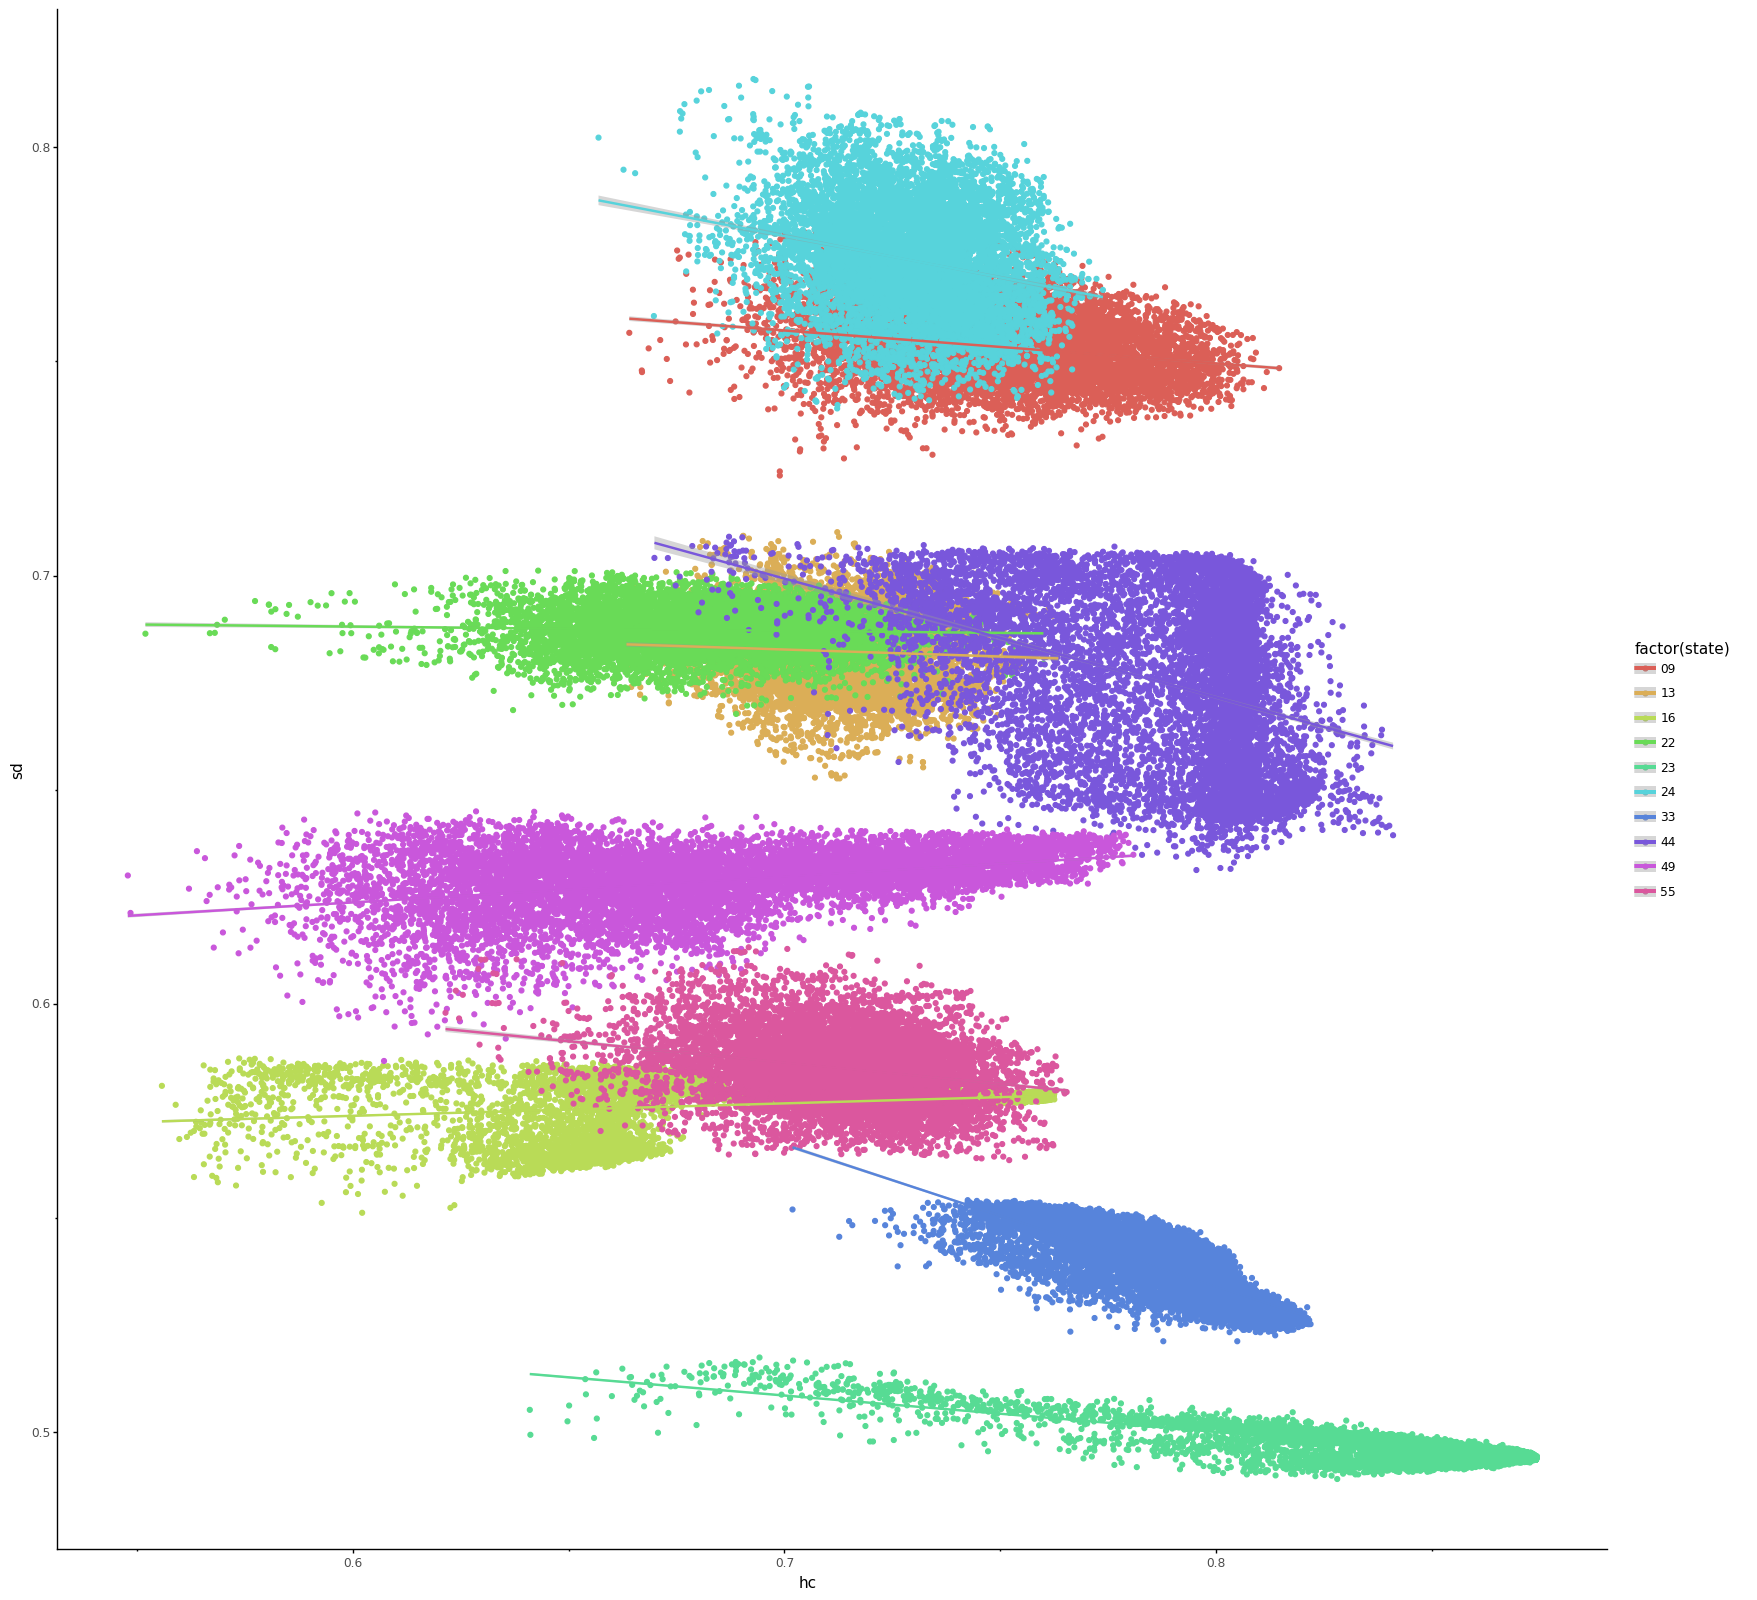
\includegraphics{../30_results/individual_regressions.png}
\caption{The individual-level regressions show a weak downward trend
between human compactness and spatial diversity\label{indiv_reg}}
\end{figure}

\begin{figure}
\centering
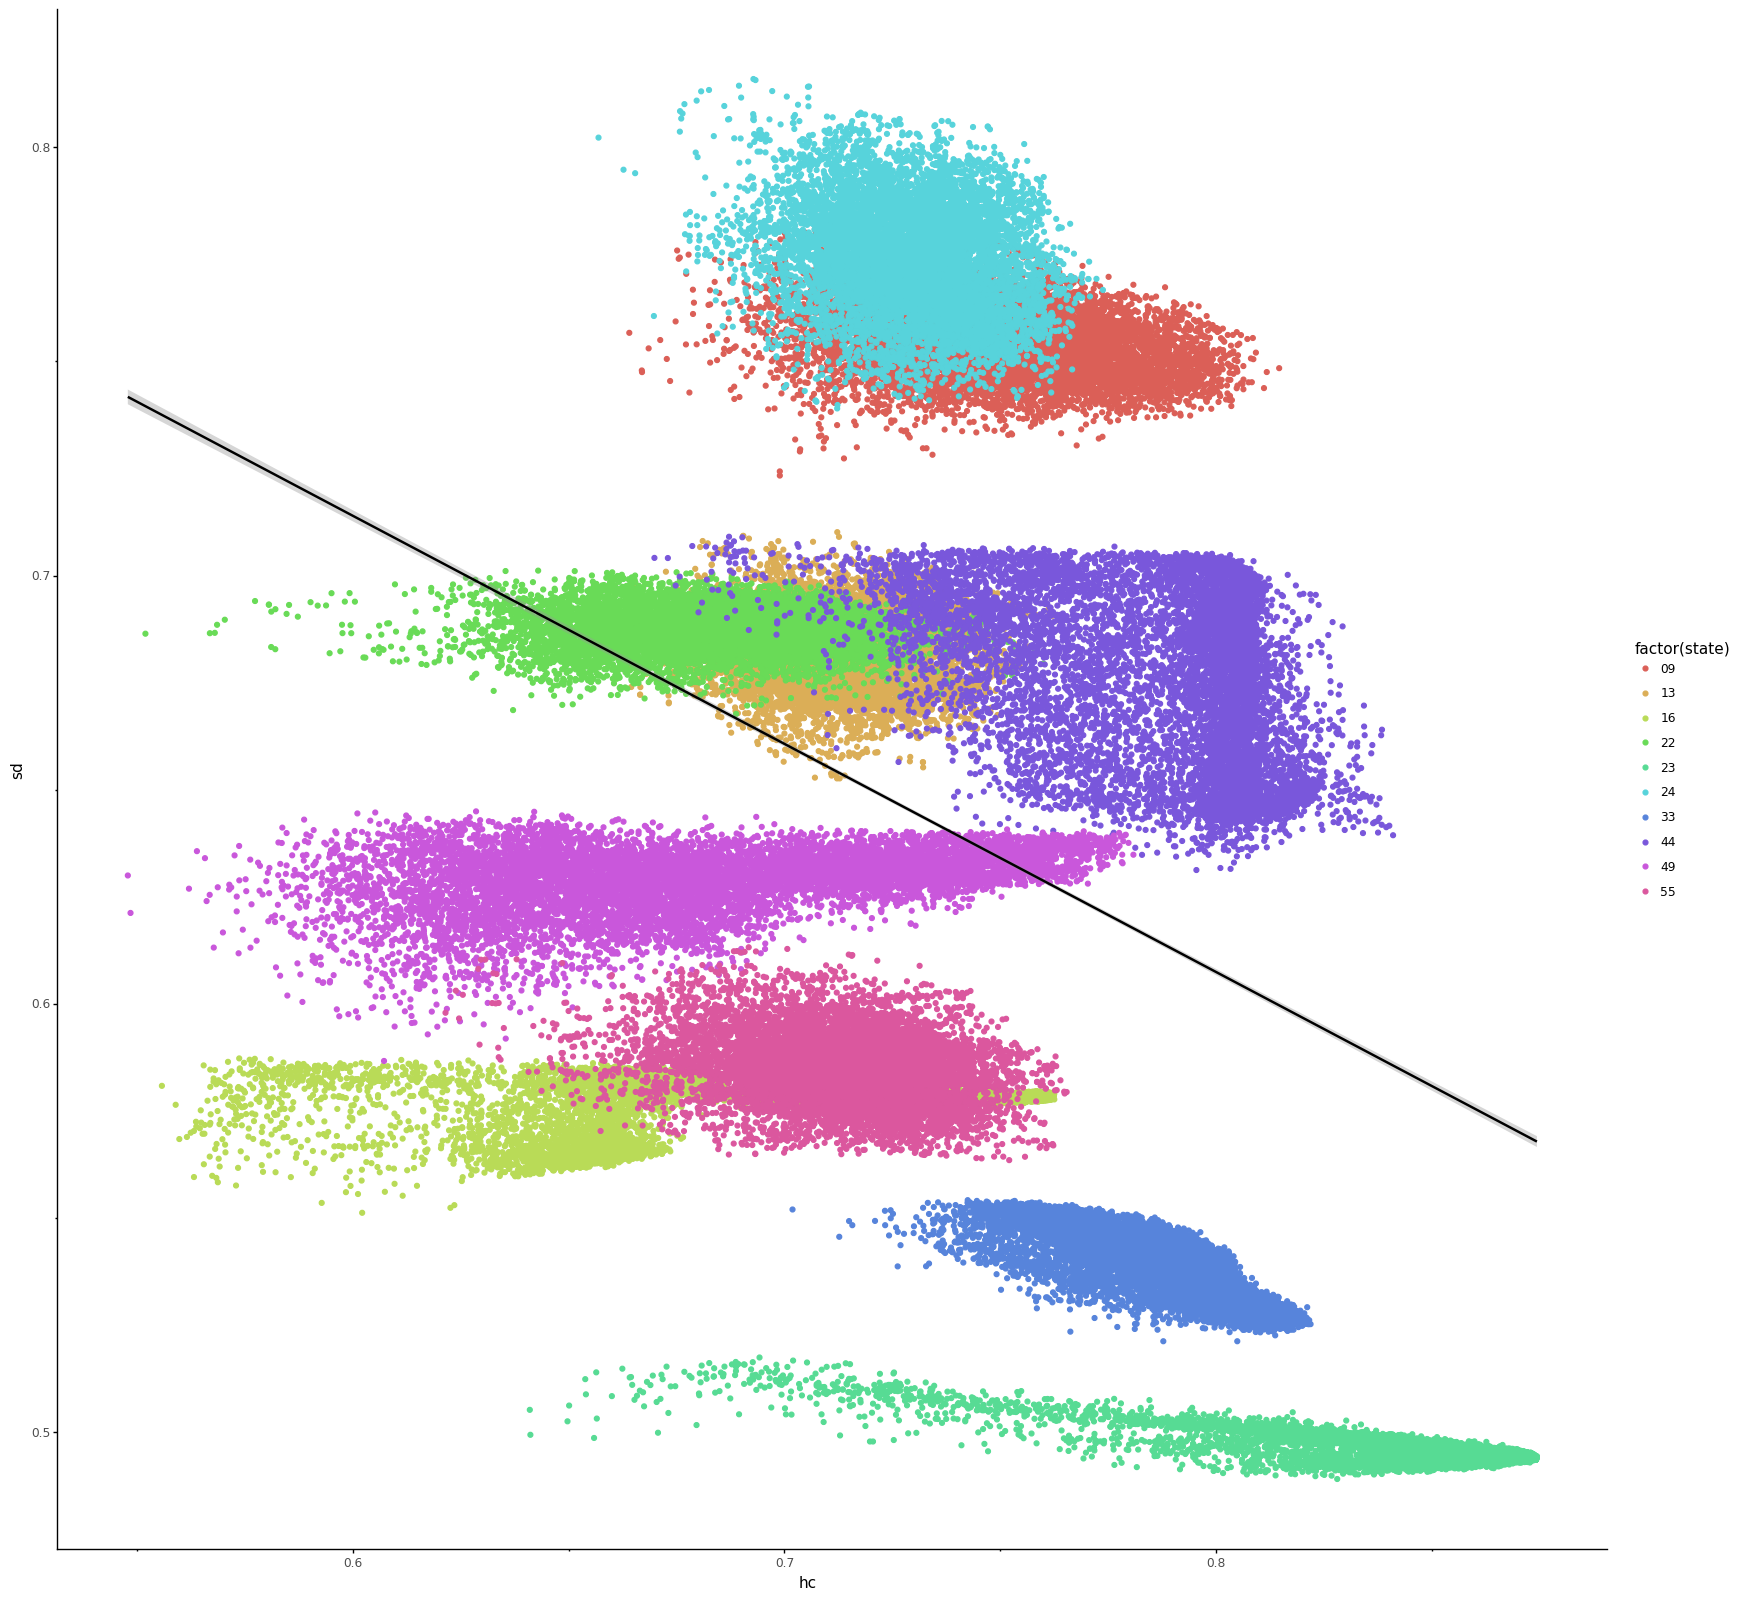
\includegraphics{../30_results/grouped_regressions.png}
\caption{Aggregating the individual states gives an inflated estimate of
the effect of compactness and commits the ecological fallacy
\label{grouped_reg}}
\end{figure}

\begin{table}[h!]
\begin{center}
\begin{tabular}{lclc}
\toprule
\textbf{Dep. Variable:}    &        sd        & \textbf{  R-squared:         } &     0.988   \\
\textbf{Model:}            &       OLS        & \textbf{  Adj. R-squared:    } &     0.988   \\
\textbf{Method:}           &  Least Squares   & \textbf{  F-statistic:       } & 8.188e+05   \\
\textbf{Date:}             & Tue, 10 Mar 2020 & \textbf{  Prob (F-statistic):} &     0.00    \\
\textbf{Time:}             &     16:04:33     & \textbf{  Log-Likelihood:    } & 3.2365e+05  \\
\textbf{No. Observations:} &      100000      & \textbf{  AIC:               } & -6.473e+05  \\
\textbf{Df Residuals:}     &       99989      & \textbf{  BIC:               } & -6.472e+05  \\
\textbf{Df Model:}         &          10      & \textbf{                     } &             \\
\bottomrule
\end{tabular}
\begin{tabular}{lcccccc}
                           & \textbf{coef} & \textbf{std err} & \textbf{t} & \textbf{P$> |$t$|$} & \textbf{[0.025} & \textbf{0.975]}  \\
\midrule
\textbf{Intercept}         &       0.7837  &        0.001     &  1042.069  &         0.000        &        0.782    &        0.785     \\
\textbf{C(district)[T.13]} &      -0.0725  &        0.000     &  -520.351  &         0.000        &       -0.073    &       -0.072     \\
\textbf{C(district)[T.16]} &      -0.1783  &        0.000     & -1255.474  &         0.000        &       -0.179    &       -0.178     \\
\textbf{C(district)[T.22]} &      -0.0687  &        0.000     &  -460.458  &         0.000        &       -0.069    &       -0.068     \\
\textbf{C(district)[T.23]} &      -0.2533  &        0.000     & -1540.668  &         0.000        &       -0.254    &       -0.253     \\
\textbf{C(district)[T.24]} &       0.0194  &        0.000     &   142.303  &         0.000        &        0.019    &        0.020     \\
\textbf{C(district)[T.33]} &      -0.2132  &        0.000     & -1534.138  &         0.000        &       -0.213    &       -0.213     \\
\textbf{C(district)[T.44]} &      -0.0763  &        0.000     &  -549.486  &         0.000        &       -0.077    &       -0.076     \\
\textbf{C(district)[T.49]} &      -0.1276  &        0.000     &  -843.636  &         0.000        &       -0.128    &       -0.127     \\
\textbf{C(district)[T.55]} &      -0.1698  &        0.000     & -1216.197  &         0.000        &       -0.170    &       -0.170     \\
\textbf{hc}                &      -0.0404  &        0.001     &   -40.632  &         0.000        &       -0.042    &       -0.038     \\
\bottomrule
\end{tabular}
\begin{tabular}{lclc}
\textbf{Omnibus:}       & 3979.140 & \textbf{  Durbin-Watson:     } &    1.171  \\
\textbf{Prob(Omnibus):} &   0.000  & \textbf{  Jarque-Bera (JB):  } & 9332.569  \\
\textbf{Skew:}          &  -0.236  & \textbf{  Prob(JB):          } &     0.00  \\
\textbf{Kurtosis:}      &   4.420  & \textbf{  Cond. No.          } &     53.4  \\
\bottomrule
\end{tabular}
\caption{OLS Regression of Spatial Diversity on Human Compactness with
Country Dummies}
\label{table:ols_sd_hc}
\end{center}
\end{table}

\hypertarget{the-most-compact-plans-have-better-spatial-diversity-than-average}{%
\subsubsection{The most compact plans have better spatial diversity than
average}\label{the-most-compact-plans-have-better-spatial-diversity-than-average}}

I therefore consider the top 500 plans

I run a differences-in-means test using Welch's t-test, as Student's
t-test relies on a homogeneity in variances assumption. When the
assumption of equal variances is not met, Student's t-test yields
unreliable results, while Welch's t-test controls Type 1 error rates as
expected. \cite{delacre2017}

I find a very strong result that

This result is even more robust than one would expect, because

\begin{verbatim}
Mean SD of plans with highest Human Compactness scores: 0.635558
Mean SD of plans with highest Polsby-Popper scores: 0.640954
Mean SD of plans with highest Reock scores: 0.639897
Mean SD of plans with highest Convex Hull scores: 0.639985
Mean SD of all plans: 0.66879
\end{verbatim}

\begin{verbatim}
Ttest_indResult(statistic=array([-26.95882013]), pvalue=array([4.92355005e-150]))
Ttest_indResult(statistic=array([-23.01140913]), pvalue=array([1.00564593e-111]))
Ttest_indResult(statistic=array([-23.65074847]), pvalue=array([1.33953995e-117]))
Ttest_indResult(statistic=array([-23.36762755]), pvalue=array([5.64959214e-115]))
\end{verbatim}

\hypertarget{the-average-spatial-diversity-of-top-plans-under-human-compactness-is-significantly-lower-than-the-average-spatial-diversity-of-top-plans-under-other-compactness-metrics}{%
\subsubsection{The average spatial diversity of top plans under human
compactness is significantly lower than the average spatial diversity of
top plans under other compactness
metrics}\label{the-average-spatial-diversity-of-top-plans-under-human-compactness-is-significantly-lower-than-the-average-spatial-diversity-of-top-plans-under-other-compactness-metrics}}

Do a t-test

Means:

\begin{verbatim}
Mean SD of top plans under Human Compactness: 0.635558
Mean SD of top plans under Polsby-Popper: 0.640954
Mean SD of top plans under Reock: 0.639897
Mean SD of top plans under Convex Hull: 0.639985
\end{verbatim}

Top 10\%:

Top 5\%:

\begin{verbatim}
Ttest_indResult(statistic=array([-3.16361084]), pvalue=array([0.00156292]))
Ttest_indResult(statistic=array([-2.53127357]), pvalue=array([0.01138011]))
Ttest_indResult(statistic=array([-2.57101923]), pvalue=array([0.0101543]))
\end{verbatim}

Top 2\%:

\hypertarget{appendix-a}{%
\section{Appendix A}\label{appendix-a}}

\hypertarget{appendix-b-results-of-difference-in-means-tests-for-individual-states}{%
\section{Appendix B: Results of difference-in-means tests for individual
states}\label{appendix-b-results-of-difference-in-means-tests-for-individual-states}}

Here I compare the average spatial diversity of all 10,000 plans per
state to the average spatial diversity of the 500 most compact plans per
state.

I present the results for each state and each metric in the ensemble,
using Welch's t-test.

\begin{verbatim}
0 Connecticut
hc
Ttest_indResult(statistic=array([-6.49740127]), pvalue=array([8.53280274e-11]))
pp
Ttest_indResult(statistic=array([0.86781049]), pvalue=array([0.3855318]))
reock
Ttest_indResult(statistic=array([0.83762575]), pvalue=array([0.40227492]))
ch
Ttest_indResult(statistic=array([-1.68248732]), pvalue=array([0.09251047]))
1 Georgia
hc
Ttest_indResult(statistic=array([-1.88909516]), pvalue=array([0.05904629]))
pp
Ttest_indResult(statistic=array([-3.3741558]), pvalue=array([0.00075958]))
reock
Ttest_indResult(statistic=array([0.39887338]), pvalue=array([0.69005064]))
ch
Ttest_indResult(statistic=array([-3.13625521]), pvalue=array([0.00174518]))
2 Idaho
hc
Ttest_indResult(statistic=array([10.42666125]), pvalue=array([2.16882037e-25]))
pp
Ttest_indResult(statistic=array([5.86780509]), pvalue=array([4.9782383e-09]))
reock
Ttest_indResult(statistic=array([5.33166925]), pvalue=array([1.24215121e-07]))
ch
Ttest_indResult(statistic=array([0.03089443]), pvalue=array([0.9753569]))
3 Louisiana
hc
Ttest_indResult(statistic=array([-3.55779128]), pvalue=array([0.00037512]))
pp
Ttest_indResult(statistic=array([-3.21856506]), pvalue=array([0.00129316]))
reock
Ttest_indResult(statistic=array([-1.77611238]), pvalue=array([0.07574051]))
ch
Ttest_indResult(statistic=array([-2.95273326]), pvalue=array([0.00315286]))
4 Maine
hc
Ttest_indResult(statistic=array([-13.2240253]), pvalue=array([9.28561364e-40]))
pp
Ttest_indResult(statistic=array([24.8919901]), pvalue=array([3.52063173e-110]))
reock
Ttest_indResult(statistic=array([11.72570569]), pvalue=array([1.36024936e-31]))
ch
Ttest_indResult(statistic=array([-13.6832433]), pvalue=array([1.9646117e-42]))
5 Rhode_Island
hc
Ttest_indResult(statistic=array([-26.07171472]), pvalue=array([3.68436833e-134]))
pp
Ttest_indResult(statistic=array([13.82562159]), pvalue=array([8.51520228e-42]))
reock
Ttest_indResult(statistic=array([5.01734031]), pvalue=array([5.92797527e-07]))
ch
Ttest_indResult(statistic=array([5.64708581]), pvalue=array([1.93856794e-08]))
6 Maryland
hc
Ttest_indResult(statistic=array([-7.72406455]), pvalue=array([1.8720555e-14]))
pp
Ttest_indResult(statistic=array([-10.69599062]), pvalue=array([7.44090023e-26]))
reock
Ttest_indResult(statistic=array([-11.43688714]), pvalue=array([2.07114299e-29]))
ch
Ttest_indResult(statistic=array([-2.44035376]), pvalue=array([0.01480235]))
7 New_Hampshire
hc
Ttest_indResult(statistic=array([-77.79139703]), pvalue=array([0.]))
pp
Ttest_indResult(statistic=array([5.66328049]), pvalue=array([2.13182847e-08]))
reock
Ttest_indResult(statistic=array([-5.62644692]), pvalue=array([2.32800657e-08]))
ch
Ttest_indResult(statistic=array([10.76371698]), pvalue=array([4.81248181e-25]))
8 Utah
hc
Ttest_indResult(statistic=array([18.41406631]), pvalue=array([8.86499654e-75]))
pp
Ttest_indResult(statistic=array([8.17458673]), pvalue=array([3.54250317e-16]))
reock
Ttest_indResult(statistic=array([6.8129706]), pvalue=array([1.05271654e-11]))
ch
Ttest_indResult(statistic=array([7.40371108]), pvalue=array([1.49308888e-13]))
9 Wisconsin
hc
Ttest_indResult(statistic=array([-6.45251298]), pvalue=array([1.16333085e-10]))
pp
Ttest_indResult(statistic=array([-2.37112098]), pvalue=array([0.01776865]))
reock
Ttest_indResult(statistic=array([-0.73082387]), pvalue=array([0.46492516]))
ch
Ttest_indResult(statistic=array([-2.87931061]), pvalue=array([0.00400501]))
\end{verbatim}

\hypertarget{very-similar-paper}{%
\subsection{Very similar paper}\label{very-similar-paper}}

We posit that this is due to thepolitical geographies of the two states,
and examining this effect isan important thread for understanding what
kinds of reforms mightor might not be effective in various
jurisdictions. Future work coulduse more sophisticated mathematical and
statistical techniques todescribe a relationship between political
geography and the trade-offs we consider here. Our analysis suggests
that a one-size-fits-allapproach to drawing `fair' districts is
inappropriate and that indi-vidual states and localities should
carefully consider the relevanttrade-offs when redistricting or
implementing redistricting reforminitiatives. One factor ignored in this
analysis, which is critical to theprocess of drawing districts,
isrespecting communities-of-interest.Even defining and locating
geographically such communities is avery difficult problem, let alone
the determination of whether ornot to preserve that group in a single
district. We therefore pro-pose our analysis as a framework for
discussion about trade-offs inredistricting rather than as a policy
recommendation.In this work, we have demonstrated with a simple model
thatdemanding districts be drawn to be as compact as possible
anddemanding that they satisfy a notion of partisan symmetry
areincompatible, but to different degrees depending on the
particularfeatures of the geographic region in question. Since existing
propos-als and methodologies for automated and algorithmic
redistrictinginvolve finding an approximate solution to an optimization
problem,it is important to understand how changing the objective
functionof these procedures can affect the outcome. As more
jurisdictionsconsider redistricting reforms, they should be cautious
about abdi-cating the line drawing process to algorithms which encode
valuesdifferent from those of the voters who use the districts to elect
theirrepresentatives.

\bibliography{references.bib}

\end{document}
